%\begin{figure}[h]
%    \centering
%	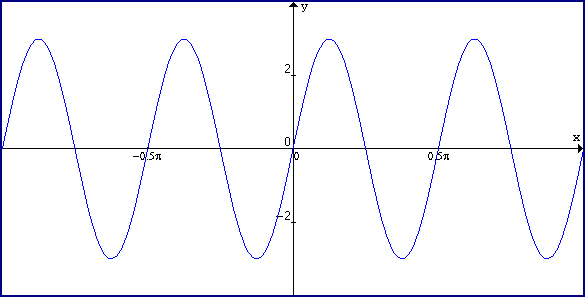
\includegraphics[scale=0.5]{graph}
%	\caption{An example graph}
%	\label{fig:x sine graph}
%\end{figure}


\newcommand{\featcount}{V}
\newcommand{\traj}{y}
\newcommand{\embed}{\vect{v}}
\newcommand{\df}{DF}
\newcommand{\featset}{\text{M}}
\newcommand{\cost}{\text{C}}

\newcommand{\semsim}{\text{Sim}}
\newcommand{\featsim}{\text{JSD}}

\newcommand{\bowmat}{\mat{B}}
\newcommand{\dtdmat}{\mat{D}}
\newcommand{\trajmat}{\mat{T}}


The core of this algorithm is taken from \cite{event-detection}. The goal of this section is to discover sets of word features highly correlated both semantically and in the time domain. The assumption is that if a group of words suddenly appears with higher frequency in a given time window and has similar meaning, it concerns the same real world event. If we extract a sample of meaningful words out of those, they can be used to represent the events. Using these words, we can query the document collection to obtain document representation of the events as well.


\section{Binary bag of words model}
To vectorize the documents, we define a matrix $\bowmat \in \left\{ 0, 1 \right\}^{\doccount \times \featcount}$, where $\featcount$ is the total vocabulary size. The document collection can then be interpreted as a set of $\doccount$ observations, each consisting of $\featcount$ binary features. The matrix $\bowmat$ is defined as

\begin{equation} \label{eq:bow-matrix}
	\bowmat_{ij} \coloneqq
	\begin{cases}
		1, & \text{document}~i~\text{contains the feature}~j \text{;} \\
		0, & \text{otherwise.}
	\end{cases}
\end{equation}

{\color{red} TODO: Figure out the min\_freq and max\_freq of words to keep.}

To limit the feature space, we trim the words appearing in less than 30 documents or in more than 90\% of the documents. The idea behind this is that the words appearing only in few documents cannot possibly represent relevant events, and are mostly anomalies. On the other hand, words appearing in most of the documents are likely stopwords, and do not carry much information. This helps to prune the feature space and makes $\bowmat$ reasonably sized.

From now on, we focus our analysis on the individual word features rather than whole documents.


\section{Computing feature trajectories}
The previous section represented word features in the document domain. This section focuses on representing these features in the time domain.

The time trajectory of a feature $f$ is a vector $\vect{\traj}_f = \left[ \traj_{f}(1), \traj_{f}(2), \dots, \traj_{f}(\streamlen) \right]$. Each element $\traj_{f}(t)$ represents the relative frequency of the feature $f$ at time $t$. This frequency is defined using the DFIDF score:

\begin{equation}
	\traj_{f}(t) \coloneqq \underbrace{\frac{\text{\df}_{f}(t)}{\text{\doccount}(t)}}_{\text{DF}} \times \underbrace{\log{\frac{\doccount}{\text{\df}_{f}}}}_{\text{IDF}},
\end{equation}

where $\text{\df}_{f}(t)$ is the number of documents published on day $t$ containing the feature $f$ (time-local document frequency), $\text{\doccount}(t)$ is the number of documents published on day $t$ and $\text{\df}_{f}$ is the number of documents containing the feature $f$ (global document frequency).

These feature trajectories are stored in a matrix $\trajmat \in \R^{\featcount \times \streamlen}$, with $\vect{\traj}_f$ being the $f$-th row of $\trajmat$. Here we take advantage of the normalization of the publication days, since they can now be used as column indices of $\trajmat$.

To make the computation efficient, we vectorize most of the operations. Along with the matrix $\bowmat$ defined in \ref{eq:bow-matrix}, we define a matrix $\dtdmat \in \left\{ 0, 1 \right\}^{\doccount \times \streamlen}$ mapping the documents to their publication days:

\begin{equation}
	\dtdmat_{ij} \coloneqq
	\begin{cases}
		1, & \text{document}~i~\text{was published on day}~j \text{;} \\
		0, & \text{otherwise}.
	\end{cases}
\end{equation}

Next, we sum the rows of $\bowmat$ together to obtain $\vect{\df} = \left[ \text{\df}_{1}, \text{\df}_{2}, \dots, \text{\df}_{\featcount} \right]$, and similarly the rows of $\dtdmat$ to obtain $\vect{\doccount}_{t} = \left[ \text{\doccount}(1), \text{\doccount}(2), \dots, \text{\doccount}(\streamlen) \right]$.

Using these matrices and vectors, we can compute $\trajmat$ as follows:

\begin{equation}
	\trajmat \coloneqq
		\underbrace{\text{diag} \left( \log{\frac{\doccount}{\vect{\df}}} \right)}_{\text{IDF}}
		\times
		\underbrace{\bowmat^{\T}
		\times \dtdmat
		\times \text{diag} \left( \frac{1}{\vect{\doccount}_{t}} \right)}_{\text{DF}}
\end{equation}


\section{Spectral analysis}
The next step is to employ spectral analysis techniques to discover periodicities in the features. Results from this section are further used to categorize the word features by their periodicity and signal power.

We apply the discrete Fourier transform to each feature trajectory, which represents the time series as a linear combination of $\streamlen$ complex sinusoids. We obtain $\mathcal{F} \vect{\traj}_{f} = \left[ X_{1}, X_{2}, \dots, X_{\streamlen}\right ]$ such that

\begin{equation*}
	X_{k} = \sum_{t = 1}^{\streamlen}{\traj_{f}(t) \exp(- \frac{2 \pi \mi}{\streamlen} (k - 1) t}), ~ k = 1, 2, \dots, \streamlen.
\end{equation*}

The absolute value of the Fourier coefficient $X_{k}$ denotes the amplitude of the complex sinusoid at frequency $\frac{k}{\streamlen}$.

Having moved from the time domain to the frequency domain, we can now analyze the signal power and dominant periodicity of each feature.

We observe peaks in the power spectrum of the transformed data and obtain the signal power and periodicity from those. The power spectrum is estimated using the periodogram estimator

\begin{equation*}
	\vect{P} = \left[ \|X_{1}\|^{2}, \|X_{2}\|^{2}, \dots, \|X_{\ceil{\streamlen / 2}}\|^{2} \right].
\end{equation*}

To measure the overall signal power, we define the dominant power spectrum of the feature $f$ as the value of the highest peak in the power spectrum, that is

\begin{equation}
	\text{DPS}_{f} \coloneqq \max\limits_{k \leq \ceil{\streamlen / 2}}{\|X_{k}\|^{2}}.
\end{equation}

The dominant period is then defined as the inverse of the frequency corresponding to the highest peak:

\begin{equation}
	\text{DP}_{f} \coloneqq \frac{\streamlen}{\argmax\limits_{k \leq \ceil{\streamlen / 2}}{\|X_{k}\|^{2}}},
\end{equation}

When applied to rows of the matrix $\trajmat$, this method yields two vectors $\vect{DPS},\ \vect{DP} \in \R^{\featcount}$, containing the dominant power spectra and dominant periods, respectively.


\section{Feature categorization}
Based on the dominant power spectra and dominant periods, we divide the features into \underline{H}igh power-\underline{H}igh period and \underline{H}igh power-\underline{L}ow period categories \footnote{\cite{event-detection} actually define \textit{five} such categories; however, our method uses only the two sets of the most powerful features.}:

\begin{equation}
\begin{split}
	\text{HH} \coloneqq \left\{ f \mid \text{DPS}_{f} > \textit{dps-bound}, \text{DP}_{f} > \ceil{\streamlen / 2} \right\}, \\
	\text{HL} \coloneqq \left\{ f \mid \text{DPS}_{f} > \textit{dps-bound}, \text{DP}_{f} \leq \ceil{\streamlen / 2} \right\}.
\end{split}
\end{equation}

{\color{red}TODO: Define dps-bound!}


\section{Event detection}
We need to define a feature similarity measure for the time domain as well as the semantic domain. These similarity measures are first defined pairwise, then generalized to a set of features, and finally connected into a single cost function.

The aperiodic and periodic features are detected separately, since we assume no connection between aperiodic events and the periodic ones.


\subsection{Measuring trajectory similarity}

Similarity between two feature trajectories is defined in terms of their information divergence. Unlike \cite{event-detection}, we use the \textit{Jensen-Shannon} divergence:

\begin{equation*}
	\featsim \left( \vect{p} \| \vect{q} \right) = \frac{1}{2} \text{D} \left( \vect{p} \| \vect{m} \right) + \frac{1}{2} \text{D} \left( \vect{q} \| \vect{m} \right),
\end{equation*}

where $\vect{m} = \frac{1}{2} \left( \vect{p} + \vect{q} \right)$ and D denotes the \textit{Kullback-Leibler} divergence.

The JS-divergence is symmetric, and its square root is a proper metric.

In the event detection algorithm, we will iteratively construct a set of highly correlated word features. When deciding which feature to add next, we will need to compute a similarity of the feature with respect to the whole set constructed so far. The trajectory similarity is generalized to a set of feature $\featset$ and a feature $f$ as

\begin{equation}
	\featsim \left( \featset, f \right) = \featsim \left( \vect{\bar{\traj}}_{\featset} \| \vect{\traj}_{f} \right),
\end{equation}

where $\vect{\bar{\traj}}_{\featset}$ is the mean of all trajectories of features in $\featset$ and $\vect{\traj}_{f}$ is the trajectory of feature f.

{\color{red} TODO: Move the pairwise similarities to the cluster-based algorithm, keep only the set-feature ones here.}

{\color{blue} TODO: Try KL(mean(M),f) instead of JSD(mean(M),f)? Like M is the true distribution and f assumed. Keep JSD in pairwise similarity though, clustering likes symmetry.}


\subsection{Measuring semantic similarity}

The semantic similarity is again first defined for two features, and then generalized to a similarity between a feature set and a new feature. Here, we utilize the word embeddings computed in \ref{word-embeddings}.

Most of the astounding results of the Word2Vec model come from semantic relations between words preserved under vector arithmetic, with angle between word vectors roughly corresponding to a topic. Thus, similarity between two features $f_{i}$ and $f_{j}$ with vector embeddings $\embed_{i}$ and $\embed_{j}$, respectively, is defined in terms of their cosine similarity as

\begin{equation}
	\semsim \left( f_{i}, f_{j} \right) \coloneqq \frac{\embed_{i} \cdot \embed{j}}{\| \embed_{i} \| \| \embed_{j} \|}
\end{equation}

The similarity is again generalized to a set of features $\featset$ and a feature $f$ as

\begin{equation}
	\semsim \left( \featset, f \right) \coloneqq \semsim \left( \bar{\embed}_{\featset}, \embed_{f} \right),
\end{equation}

where $\bar{\embed}_{\featset}$ is the mean of all vector embeddings of features in $\featset$ and $\embed_{f}$ is the vector embedding of the feature $f$. Here, the mean vector is supposed to represent a shared topic among words from $\featset$.


\subsection{Event detection}

We can now measure the similarity of a feature set both in the time domain (using JS-divergence) and in the semantic domain (using semantic similarity). These two measures are combined into a cost function $\cost$, which we aim to minimize.

\begin{equation} \label{eq:cost-function}
	\cost \left( \featset, f \right) \coloneqq \frac{\featsim \left( \featset, f \right)}{\exp(\semsim \left( \featset, f \right)) \cdot \sum_{g \in \featset \cup f}{\text{DPS}_{g}}}
\end{equation}

We exponentiate the cosine similarity so that the resulting value is always positive. Intuitively, a set $\featset \cup f$ which minimizes this function will have low inter-trajectory divergence, high semantic similarity and will be comprised of relevant features with high DPS.

To perform the event detection itself, we mostly adapt the \textit{Unsupervised greedy event detection} algorithm from \cite{event-detection}.

\begin{algorithm}[H]
\begin{algorithmic}[1]
\caption{Unsupervised greedy event detection}
\Input $\text{Feature set} ~ \featset \coloneqq \text{HH or HL}$

\State $\text{Sort the features in ascending DPS order: } DPS_{f_{1}} \leq DPS_{f_{2}} \leq \dots \leq DPS_{f_{\left\vert M \right\vert}}$

\State $k = 0$

\ForEach{$f \in \featset$}
	\State $k = k + 1$	
	\State $e_{k} = \{ f \}$
	\State $\cost_{e_{k}} = \frac{1}{DPS_{f}}$
	\State $\featset = \featset \setminus f$
	
	\While{$M \neq \emptyset$}
		\State $m = \argmin\limits_{m}{\cost \left( e_{k}, f_{m} \right)}$

		\If{$\cost \left( e_{k}, f_{m} \right) < \cost_{e_{k}}$}
			\State $\cost_{e_{k}} = \cost \left( e_{k}, f_{m} \right)$
			\State $e_{k} = e_{k} \cup f_{m}$
			\State $\featset = \featset \setminus f_{m}$
		\Else
			\Break
		\EndIf
	\EndWhile
\EndFor

\Output $\{ e_{1}, e_{2}, \dots, e_{k} \}$
\end{algorithmic}
\end{algorithm}

We do make two changes, however. First, we sort the features in \textit{ascending} rather than descending order. This ensures that words with lower DPS value will get selected first and that the function \ref{eq:cost-function} will not be minimized as quickly. As a result, the events will contain more representing features and will not be broken into several events concerning the same real-world event. This effectively relaxes the DPS part of the function \ref{eq:cost-function} while keeping emphasis on the trajectory similarity and document overlap.

Second, we output the events as sets of word features rather than event trajectories. This is simply because we will need to access the individual features, and later, documents, of each event.